% !TeX program = xelatex
% ============================================================
%  《系统开发工具基础》实验报告 —— 第 4 周
%  姓名：徐宜安  学号：25060012033
%  编译：latexmk -xelatex 实验报告.tex
% ============================================================
\documentclass[12pt,a4paper,fontset=fandol]{ctexart}

% ---------- 页面布局 ----------
\usepackage[a4paper,margin=2.3cm]{geometry}
\setlength{\headheight}{14pt}
\setlength{\emergencystretch}{3em}

% ---------- 数学 ----------
\usepackage{amsmath,amssymb}

% ---------- 图片 ----------
\usepackage{graphicx}
\graphicspath{{课上/q13/}{课上/q14/}{课上/q15/}{课上/q16/}}
\usepackage{caption}
\captionsetup{font=small,labelfont=bf,labelsep=quad}
\usepackage{placeins}
\usepackage{float}
\usepackage{needspace}
\makeatletter
\setlength{\@fpsep}{12pt}
\makeatother

% ---------- 表格 ----------
\usepackage{booktabs,array,multirow}

% ---------- 颜色与代码高亮 ----------
\usepackage{xcolor}
\definecolor{codebg}{HTML}{f6f8fa}
\definecolor{codeframe}{HTML}{d0d7de}
\definecolor{kwred}{HTML}{cf222e}
\definecolor{strblue}{HTML}{0a3069}
\definecolor{cmtgray}{HTML}{6e7781}
\definecolor{fnpurple}{HTML}{8250df}
\definecolor{numblue}{HTML}{0550ae}

\usepackage{listings}
\renewcommand{\lstlistingname}{代码}

\lstdefinelanguage{shell}{
  morekeywords={mkdir,cd,echo,touch,cp,rm,mv,find,chmod,pwd,ls,cat,head,tail,sort,uniq,awk,sed,grep,printf,exit,return,if,then,else,elif,fi,do,done,for,in,while,case,esac,trap,sleep,bg,jobs,kill,wait,set,export,source,local,time,python,pip,pytest,ruff,curl,jq,make,sha256sum},
  morekeywords=[2]{git,init,add,commit,checkout,merge,log,status,branch,clone,push,pull,diff,stash,restore,switch},
  morecomment=[l]{\#},
  morestring=[b]",
  morestring=[b]',
  sensitive=true,
}

\lstdefinelanguage{py}{
  morekeywords={import,from,def,return,if,else,elif,for,in,while,print,with,open,as,class,assert,raise,range,lambda},
  morecomment=[l]{\#},
  morestring=[b]",
  morestring=[b]',
  sensitive=true,
}

\lstdefinestyle{labcode}{
  backgroundcolor=\color{codebg},
  basicstyle=\small\ttfamily,
  keywordstyle=\color{kwred}\bfseries,
  keywordstyle=[2]\color{fnpurple}\bfseries,
  commentstyle=\color{cmtgray}\itshape,
  stringstyle=\color{strblue},
  numberstyle=\tiny\color{cmtgray},
  numbers=left,
  frame=single,
  rulecolor=\color{codeframe},
  breaklines=true,
  breakatwhitespace=false,
  showstringspaces=false,
  tabsize=4,
  columns=fullflexible,
  keepspaces=true,
  captionpos=b,
  xleftmargin=1.6em,
  framexleftmargin=1.2em,
  aboveskip=0.6em,
  belowskip=0.6em,
}
\lstset{style=labcode}

% ---------- 页眉页脚 ----------
\usepackage{fancyhdr}
\usepackage{lastpage}
\pagestyle{fancy}
\fancyhf{}
\fancyhead[L]{\small 系统开发工具基础 · 实验报告}
\fancyhead[R]{\small 徐宜安\quad 25060012033}
\fancyfoot[C]{\small 第 \thepage\ 页 / 共 \pageref{LastPage} 页}
\renewcommand{\headrulewidth}{0.4pt}

% ---------- 超链接 ----------
\usepackage{hyperref}
\hypersetup{colorlinks=true,linkcolor=numblue,urlcolor=numblue,citecolor=numblue}

% ---------- 题目要求框 ----------
\usepackage{tcolorbox}
\tcbuselibrary{breakable}
\newtcolorbox{taskbox}[1][]{
  colback=blue!4!white,
  colframe=blue!50!black,
  fonttitle=\bfseries,
  title={#1},
  boxrule=0.6pt,
  arc=1.5pt,
  left=8pt,right=8pt,top=5pt,bottom=5pt,
  breakable,
}

% ---------- 列表 ----------
\usepackage{enumitem}

% ==================== 每周填写区 ====================
\newcommand{\weeknum}{第 4 周}
\newcommand{\weektheme}{代码质量 · 元编程 · 大杂烩 · 课堂综合测试}
\newcommand{\classdate}{2026 年 9 月 14 日}
% ==================== 每周填写区结束 ====================

\newcommand{\makereporttitle}{%
  \begin{center}
    {\LARGE\bfseries 系统开发工具基础 · 实验报告}\\[0.4em]
    {\small \weeknum：\weektheme}\\[0.7em]
    {\small
    \begin{tabular}{@{}ll@{\hspace{3em}}ll@{}}
      姓\quad 名 & 徐宜安 & 学\quad 号 & 25060012033 \\
      授课教师 & 周小伟 & 上课日期 & \classdate \\
      Git 仓库 & \href{https://github.com/xya-123/Fundamentals-of-Computer-System-Development-Tools}{GitHub 课程仓库} & 报告日期 & \today \\
    \end{tabular}}\\[0.7em]
    \rule{\textwidth}{0.8pt}
  \end{center}
}

\begin{document}
\makereporttitle

\section{课上练习}

% ================= q13 =================
\subsection{q13 · 建立可执行的本地质量门禁（代码质量）}

\begin{taskbox}[题目要求]
复用 q10 完成的 \texttt{greetlab} 包，在 q13 中建立轻量本地质量检查：
\begin{itemize}[nosep]
  \item 在 \texttt{pyproject.toml} 中加入 Ruff 和 Pytest 的最小配置；
  \item 保留正常姓名与空白姓名两个带有效断言的测试；
  \item 运行 \texttt{ruff format}、\texttt{ruff check} 和 \texttt{pytest}，修复全部问题且不全局忽略规则；
  \item 编写 \texttt{check.sh} 依次执行三项检查，并保证返回 0。
\end{itemize}
\end{taskbox}

\textbf{实验过程：} 首先把 q10 复制为 q13，并以可编辑方式安装当前项目，同时确认
Ruff 和 Pytest 已经安装。随后在 \texttt{pyproject.toml} 中加入格式、检查规则和测试路径配置，
其中 Ruff 选择 E、F、W 三组规则，Pytest 明确从 \texttt{tests} 收集测试，并把
\texttt{src} 加入 Python 搜索路径。本题新增的核心配置如下。

\begin{lstlisting}[language=,caption={本题新增的 Ruff 与 Pytest 配置},label={lst:q13-config}]
[tool.ruff]
line-length = 120

[tool.ruff.lint]
select = ["E", "F", "W"]

[tool.pytest.ini_options]
testpaths = ["tests"]
pythonpath = ["src"]
\end{lstlisting}

第一次执行 \texttt{ruff format --check} 时，终端指出
\texttt{src/greetlab/cli.py} 和 \texttt{tests/test\_cli.py} 两个文件需要重新格式化，
具体差异是导入语句与函数之间缺少规范空行。项目复制、依赖安装和首次检查结果见图~\ref{fig:q13-first-check}。

\begin{figure}[H]
  \centering
  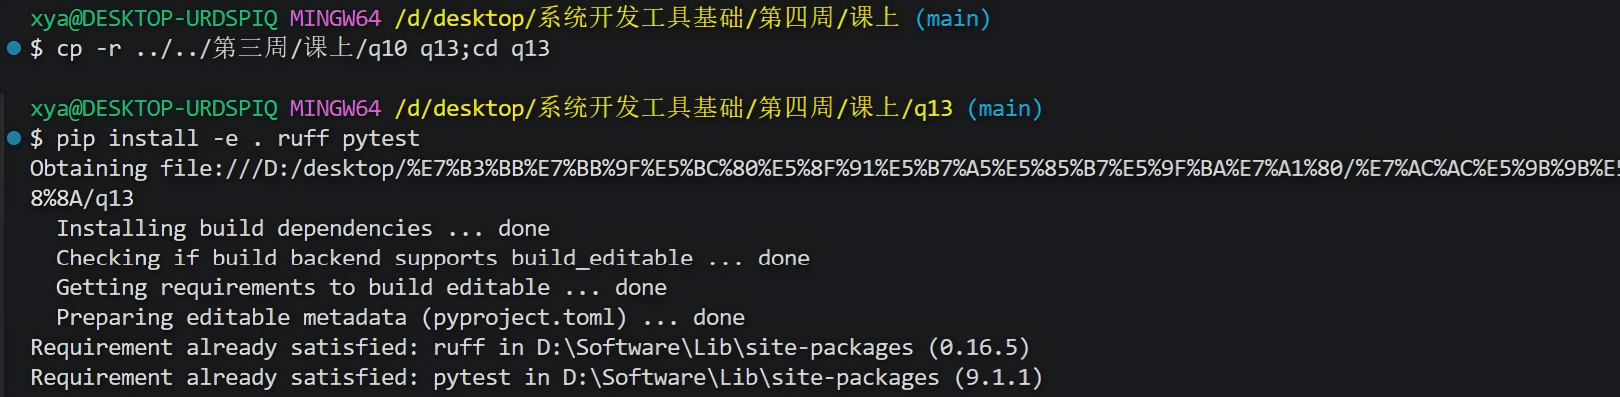
\includegraphics[width=0.96\textwidth]{课上/q13/1-安装依赖前部分.png}\\[-0.45em]
  {\small (a) 复制 q10 并安装当前项目、Ruff 与 Pytest}\\[0.15em]
  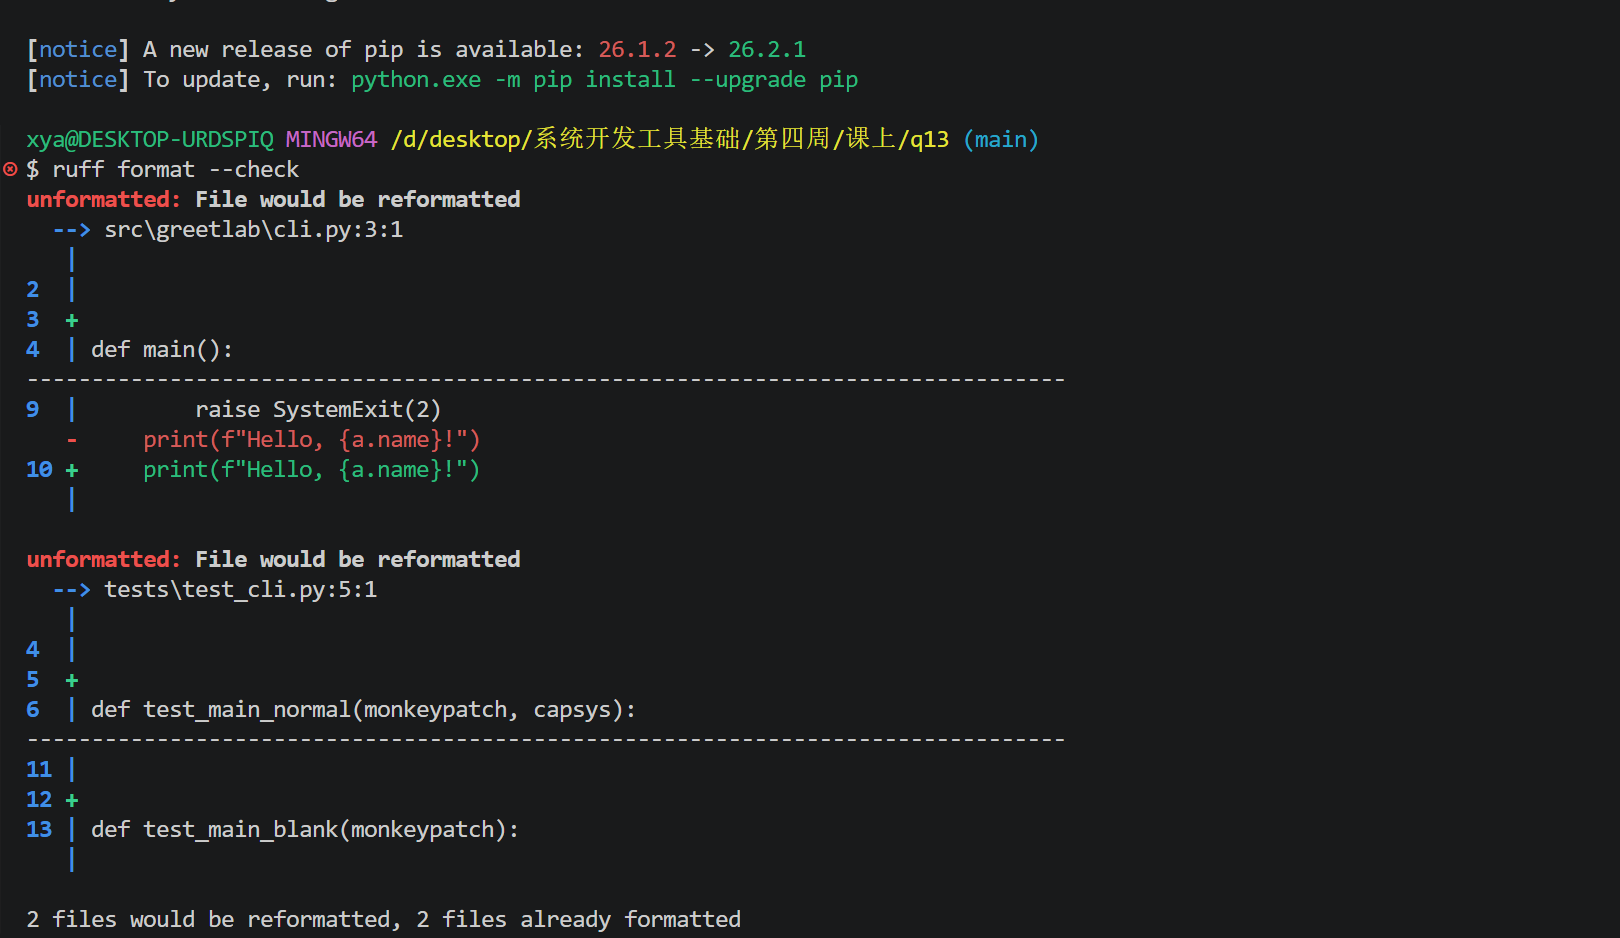
\includegraphics[width=0.96\textwidth]{课上/q13/2-安装依赖后+check.png}\\[-0.35em]
  {\small (b) 首次格式检查指出两个文件需要调整}
  \caption{q13 环境准备与首次 Ruff 格式检查}
  \label{fig:q13-first-check}
\end{figure}

执行 \texttt{ruff format .} 后两个文件被自动整理，再运行
\texttt{ruff check .} 和 \texttt{pytest}，代码检查全部通过，两个测试也均通过。
最后把三条命令写入 \texttt{check.sh}，其中 \texttt{set -euo pipefail}
保证任一检查失败时脚本立即以非零状态结束。

\lstinputlisting[language=shell,caption={依次执行格式、代码和测试检查的本地门禁},label={lst:q13-check}]{课上/q13/check.sh}

单独执行三项检查的结果见图~\ref{fig:q13-pass}(a)。为脚本增加执行权限后运行
\texttt{./check.sh}，三项检查再次通过，\texttt{echo \$?} 输出 0，见图~\ref{fig:q13-pass}(b)。

\begin{figure}[H]
  \centering
  
\includegraphics[width=0.96\textwidth]{课上/q13/3.png}\\[-0.35em]
  {\small (a) 格式化后 Ruff 检查和两个 Pytest 测试全部通过}\\[0.15em]
  
\includegraphics[width=0.96\textwidth]{课上/q13/4.png}\\[-0.35em]
  {\small (b) 运行统一检查脚本并确认退出码为 0}
  \caption{q13 修复格式问题并运行本地质量门禁}
  \label{fig:q13-pass}
\end{figure}

\textbf{实验结果：} q13 已建立可重复执行的本地质量门禁。当前代码格式、Ruff 规则和两个功能测试
全部通过，脚本正常结束并返回 0。

\FloatBarrier

% ================= q14 =================
\subsection{q14 · 让 Make 只重建真正受影响的产物（元编程：构建系统）}

\begin{taskbox}[题目要求]
根据给定的 \texttt{data.csv}、\texttt{stats.py}、\texttt{build\_report.py} 和
\texttt{report.md} 编写 Makefile：
\begin{itemize}[nosep]
  \item 包含 \texttt{all}、\texttt{stats.txt}、\texttt{report.txt} 和 \texttt{clean}；
  \item 准确列出数据文件、脚本和中间产物依赖，并将 \texttt{all}、\texttt{clean} 声明为 \texttt{.PHONY}；
  \item 验证首次构建、无改动时不执行配方，以及更新 \texttt{data.csv} 后的依赖传播；
  \item 确认 \texttt{clean} 只删除生成物。
\end{itemize}
\end{taskbox}

\textbf{实验过程：} q14 初始包含 Makefile 和题目给出的四个源文件。
\texttt{stats.txt} 依赖 \texttt{data.csv} 与 \texttt{stats.py}；
\texttt{report.txt} 除了依赖报告模板和生成脚本，还依赖前一步得到的
\texttt{stats.txt}。这样数据变化时会先重算统计值，再重建最终报告。Makefile 内容如下。

\lstinputlisting[language=shell,caption={统计结果与文本报告的构建依赖},label={lst:q14-makefile}]{课上/q14/Makefile}

第一次运行 \texttt{make} 时，Make 依次执行两个 Python 脚本，生成
\texttt{stats.txt} 和 \texttt{report.txt}，过程见图~\ref{fig:q14-build}。

\begin{figure}[H]
  \centering
  
\includegraphics[width=0.82\textwidth]{课上/q14/1.png}
  \caption{q14 首次执行 Make 并运行两个生成脚本}
  \label{fig:q14-build}
\end{figure}

统计值为 10，最终报告包含标题和 \texttt{Total: 10}，见图~\ref{fig:q14-noop}(a)。
在没有修改任何文件的情况下再次执行 \texttt{make}，终端提示
\texttt{Nothing to be done for 'all'}，没有重复运行脚本，见图~\ref{fig:q14-noop}(b)。

\begin{figure}[H]
  \centering
  
\includegraphics[width=0.94\textwidth]{课上/q14/2.png}\\[-0.35em]
  {\small (a) 统计文件与最终报告的内容}\\[0.15em]
  
\includegraphics[width=0.86\textwidth]{课上/q14/3.png}\\[-0.35em]
  {\small (b) 无改动时 Make 不重复执行配方}
  \caption{q14 构建结果与无改动时的增量检查}
  \label{fig:q14-noop}
\end{figure}

接着使用 \texttt{touch data.csv} 更新数据文件的修改时间。再次执行 \texttt{make} 时，
\texttt{stats.py} 与 \texttt{build\_report.py} 都被重新运行，说明中间产物的依赖继续传递到最终报告。
数据内容没有改变，因此两个产物的内容仍为 10。最后执行 \texttt{make clean}，只删除
\texttt{stats.txt} 和 \texttt{report.txt}；Makefile 与四个源文件均被保留。相关过程见图~\ref{fig:q14-rebuild}。

\begin{figure}[H]
  \centering
  
\includegraphics[width=0.94\textwidth]{课上/q14/4.png}
  \caption{更新数据后重新构建，并用 clean 删除两个生成物}
  \label{fig:q14-rebuild}
\end{figure}

\textbf{实验结果：} Make 能根据依赖文件的修改时间决定是否执行配方。首次构建生成两个产物，
无改动时不重复执行，数据文件更新后两个产物按依赖顺序重建，清理目标也没有删除源文件。

\FloatBarrier

% ================= q15 =================
\subsection{q15 · 把本地 API 数据转换为可读报告（API、jq 与 CLI）}

\begin{taskbox}[题目要求]
把题目给定的 JSON 保存为 \texttt{packages.json}，并完成以下操作：
\begin{itemize}[nosep]
  \item 在 q15 中运行本地 HTTP 服务，使用 \texttt{curl -fsS} 获取 JSON；
  \item 用 jq 筛选状态为 active 且下载量不少于 100 的记录；
  \item 按下载量降序、名称升序排列；
  \item 编写 \texttt{api\_report.sh}，生成包含标题与三列表格的 \texttt{summary.md}。
\end{itemize}
\end{taskbox}

\textbf{实验过程：} 首先在 q15 保存包含五条记录的 \texttt{packages.json}，
在一个终端中运行 \texttt{python -m http.server 8000}，再从另一个终端使用
\texttt{curl -fsS} 请求 \texttt{http://127.0.0.1:8000/packages.json}。
服务端记录显示请求返回 HTTP 200，客户端也成功取得并格式化显示全部 JSON，见图~\ref{fig:q15-fetch}。

\begin{figure}[H]
  \centering
  
\includegraphics[width=0.98\textwidth]{课上/q15/1.png}
  \caption{q15 启动本地 HTTP 服务并使用 curl 获取 JSON 数据}
  \label{fig:q15-fetch}
\end{figure}

随后用 jq 保留 \texttt{status} 为 \texttt{active} 且
\texttt{downloads} 不少于 100 的记录，并用负下载量与名称组成排序键。
筛选后剩下 delta、gamma、alpha 三项，下载量相同的 delta 与 gamma 按名称升序排列，
结果见图~\ref{fig:q15-filter}。

\begin{figure}[H]
  \centering
  
\includegraphics[width=0.88\textwidth]{课上/q15/2.png}
  \caption{q15 使用 jq 按条件筛选并按两个关键字排序}
  \label{fig:q15-filter}
\end{figure}

最后把获取、筛选、排序和 Markdown 行生成写进脚本。脚本先输出标题与表头，
再用 jq 的 \texttt{-r} 参数生成三行不带 JSON 引号的表格内容，核心代码如下。

\begin{lstlisting}[language=shell,caption={从本地 API 生成 Markdown 表格的核心代码},label={lst:q15-script}]
{
  echo "# Active Package Report"
  echo
  echo "| name | version | downloads |"
  echo "|---|---|---:|"
  curl -fsS "$url" | jq -r '
    [.[] | select(.status == "active" and .downloads >= 100)]
    | sort_by([-.downloads, .name]) | .[]
    | "| \(.name) | \(.version) | \(.downloads) |"
  '
} > summary.md
\end{lstlisting}

赋予脚本执行权限并运行后，生成的 \texttt{summary.md} 包含正确标题、列名和三条记录，
最终内容见图~\ref{fig:q15-summary}。

\begin{figure}[H]
  \centering
  
\includegraphics[width=0.72\textwidth]{课上/q15/3.png}
  \caption{q15 脚本生成的 Markdown 三列表格}
  \label{fig:q15-summary}
\end{figure}

\textbf{实验结果：} 本地 HTTP 服务能够正常提供 JSON 数据。脚本最终保留下载量分别为
450、450 和 120 的三条有效记录，并按 delta、gamma、alpha 的顺序生成 Markdown 表格。

\FloatBarrier

% ================= q16 =================
\Needspace{12\baselineskip}
\subsection{q16 · 修复并交付一个陌生的小型工具仓库（课堂综合测试）}

\begin{taskbox}[题目要求]
复用 q13 的项目完成一次综合检查：
\begin{itemize}[nosep]
  \item 临时把问候语实现改为固定输出 \texttt{Hello, name!}，运行质量门禁确认测试失败，再定位并修复；
  \item 编写包含 \texttt{check}、\texttt{build} 和 \texttt{clean} 的最小 Makefile；
  \item 运行 \texttt{make check} 和 \texttt{make build}，生成 wheel 并计算 SHA-256；
  \item 将最终改动提交为内容聚焦的 Git 提交。
\end{itemize}
\end{taskbox}

\textbf{实验过程：} 从 q13 复制源码、测试、项目配置和检查脚本到 q16，并继续使用课程根目录的 Git 仓库。
为了验证测试是否真正约束了程序行为，先把问候语临时改成固定字符串
\texttt{Hello, name!}。此时格式和静态检查仍然通过，但正常姓名测试得到的实际输出与期望不符，
Pytest 显示 \texttt{1 failed, 1 passed}，失败位置和差异见图~\ref{fig:q16-fail}。

\begin{figure}[H]
  \centering
  
\includegraphics[width=0.96\textwidth]{课上/q16/1.png}
  \caption{q16 临时引入固定问候语后，正常姓名测试准确失败}
  \label{fig:q16-fail}
\end{figure}

根据失败断言，把固定字符串恢复为使用 \texttt{a.name} 的格式化输出。
再次执行 \texttt{check.sh} 后两个测试均通过，退出码为 0，见图~\ref{fig:q16-fixed}(a)。
随后编写最小 Makefile：\texttt{check} 调用已有质量门禁，\texttt{build} 生成 wheel，
\texttt{clean} 只清理构建目录、分发目录和包元数据。

\lstinputlisting[language=shell,caption={质量检查、wheel 构建与清理目标},label={lst:q16-makefile}]{课上/q16/Makefile}

运行 \texttt{make check} 后，Makefile 成功调用检查脚本，格式、代码和测试检查全部通过，
结果见图~\ref{fig:q16-fixed}(b)。

\begin{figure}[H]
  \centering
  
\includegraphics[width=0.96\textwidth]{课上/q16/2.png}\\[-0.35em]
  {\small (a) 修复问候语后直接运行质量门禁}\\[0.15em]
  
\includegraphics[width=0.96\textwidth]{课上/q16/3.png}\\[-0.35em]
  {\small (b) 通过 Makefile 的 check 目标运行同一套检查}
  \caption{q16 修复后的直接检查与 Make 检查}
  \label{fig:q16-fixed}
\end{figure}

接下来执行 \texttt{make build}。构建工具创建隔离环境并打包项目，最终生成
\texttt{greetlab\_25060012033-0.1.0-py3-none-any.whl}。由于构建输出较长，
图~\ref{fig:q16-delivery}(a) 连续保留开始与成功结束两部分。随后使用
\texttt{sha256sum dist/*.whl} 计算构建产物摘要，得到
\texttt{006eb8581c99b33a48182971d20e573109202bea41ba76b16f781da68fd18f6f}，
见图~\ref{fig:q16-delivery}(b)。

最后只暂存 Makefile、检查脚本、项目配置、源码和测试文件，提交信息为
“完成 q16 综合质量检查与构建流程”。执行提交命令的记录见图~\ref{fig:q16-delivery}(c)，
Git 日志中对应提交为 \texttt{99480f6}。

\begin{figure}[H]
  \centering
  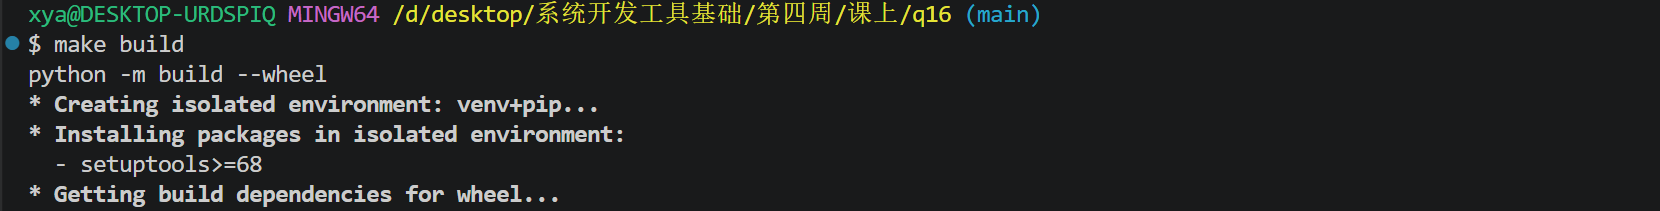
\includegraphics[width=0.96\textwidth]{课上/q16/4-build头-请和尾巴放一起.png}\\[-0.72em]
  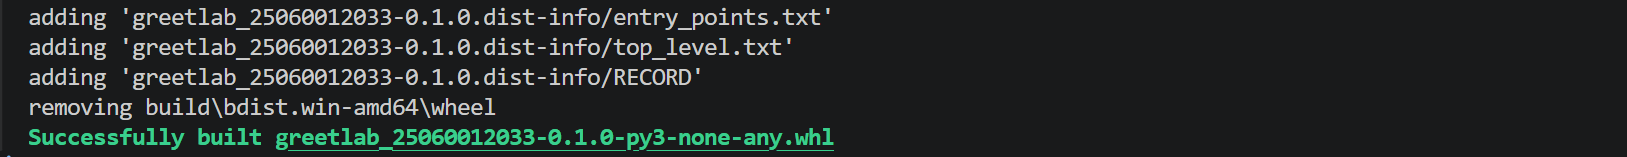
\includegraphics[width=0.96\textwidth]{课上/q16/5build尾巴.png}\\[-0.35em]
  {\small (a) wheel 构建开始与成功结束记录}\\[0.20em]
  
\includegraphics[width=0.92\textwidth]{课上/q16/6.png}\\[-0.35em]
  {\small (b) wheel 的 SHA-256 摘要}\\[0.20em]
  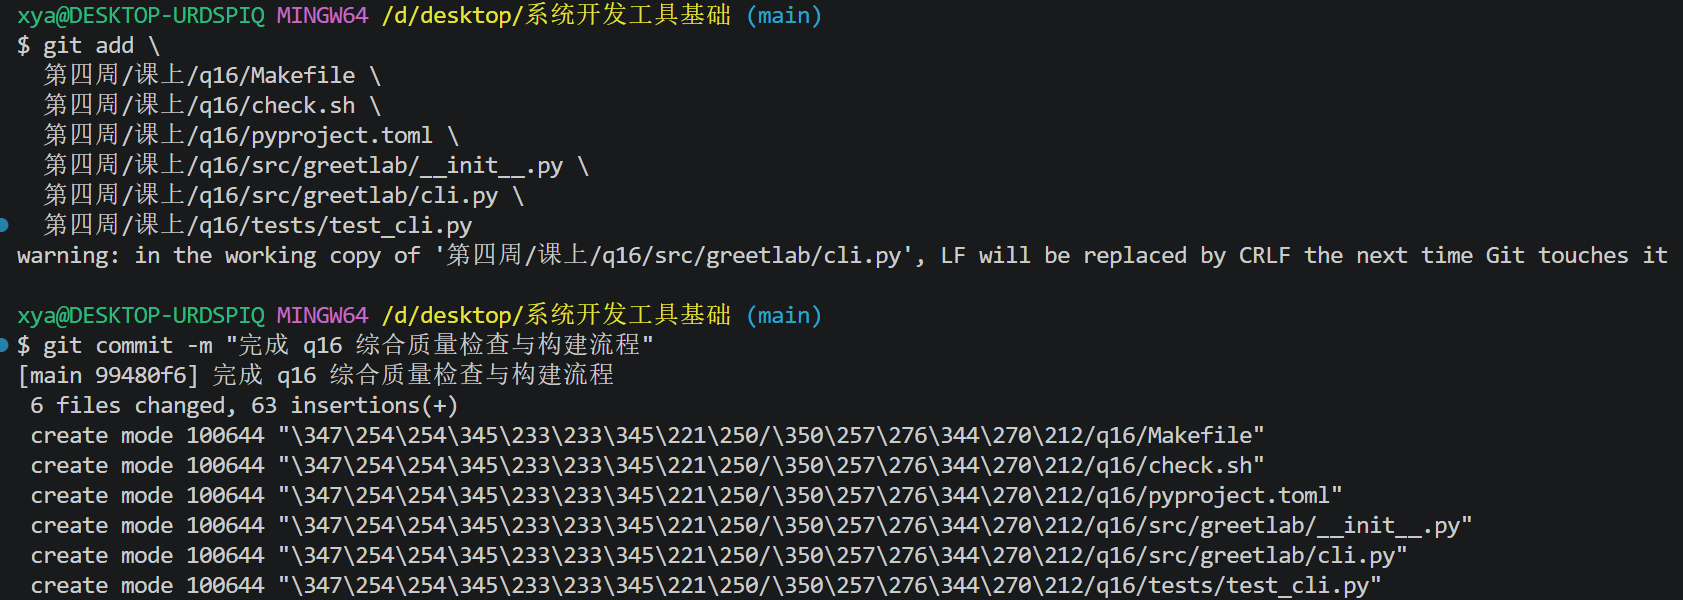
\includegraphics[width=0.96\textwidth]{课上/q16/7.png}\\[-0.35em]
  {\small (c) 只暂存核心文件并执行 Git 提交}
  \caption{q16 wheel 构建、完整性摘要与最终提交}
  \label{fig:q16-delivery}
\end{figure}

\textbf{实验结果：} 测试能够发现固定问候语带来的行为错误，修复后本地质量门禁与
\texttt{make check} 均通过；\texttt{make build} 成功生成 wheel，SHA-256 摘要计算完成，
核心代码和构建流程也已提交到 Git 仓库。

\FloatBarrier

\section{课后练习}

\paragraph{参考资料记录}
\href{https://missing-semester-cn.github.io/2026/code-quality/}{Missing Semester：代码质量}、
\href{https://missing-semester-cn.github.io/2020/metaprogramming/}{Missing Semester：元编程}、
\href{https://missing-semester-cn.github.io/2020/potpourri/}{Missing Semester：大杂烩}。

\newcommand{\afterpracticeimage}[4]{%
  \begin{figure}[H]
    \centering
    \includegraphics[width=#1\textwidth]{#2}
    \caption{#3}
    \label{#4}
  \end{figure}
}

\noindent\textbf{实例 1：用 Ruff 检查并修复嵌套判断。}
在 \texttt{nested.py} 中写入两层判断，只启用 SIM102 规则检查时，Ruff 指出两个
\texttt{if} 可以合并。普通的 \texttt{--fix} 不会应用这项修改，确认改动后加入
\texttt{--unsafe-fixes}，两个条件被合并到同一条判断中，复检通过，见图~\ref{fig:after-quality-1}。

\afterpracticeimage{0.96}{课后/quality/1.png}{Ruff 发现并修复 SIM102 问题}{fig:after-quality-1}

\noindent\textbf{实例 2：使用参数化测试覆盖多组输入。}
价格计算函数接收原价和折扣，使用 \texttt{pytest.mark.parametrize} 设置无折扣、八折和
五折三组输入。指定该测试函数运行后，三组结果均通过，见图~\ref{fig:after-quality-2}。

\afterpracticeimage{0.96}{课后/quality/2.png}{参数化测试的三组输入全部通过}{fig:after-quality-2}

\noindent\textbf{实例 3：添加并单独运行回归测试。}
针对负数价格补充回归测试，要求函数抛出带有 \texttt{non-negative} 提示的
\texttt{ValueError}。使用 \texttt{-k regression} 后，Pytest 从四项测试中只运行该项，
得到一项通过、三项未选择，见图~\ref{fig:after-quality-3}。

\afterpracticeimage{0.96}{课后/quality/3.png}{使用关键词单独运行回归测试}{fig:after-quality-3}

\noindent\textbf{实例 4：使用 Mock 模拟外部接口。}
用 \texttt{Mock} 代替接口客户端，将 \texttt{/rate} 的返回值设为 0.8，再检查函数结果和
实际调用参数。该测试不访问网络，单独运行后通过，见图~\ref{fig:after-quality-4}。

\afterpracticeimage{0.96}{课后/quality/4.png}{使用 Mock 完成不访问网络的接口测试}{fig:after-quality-4}

\noindent\textbf{实例 5：检查并提高测试覆盖率。}
用 pytest-cov 运行全部测试并生成终端与 HTML 报告。第一次运行时 \texttt{price.py}
第 5 行未覆盖，覆盖率为 88\%；加入折扣超出范围的测试后，六项测试全部通过，
遗漏行数变为 0，覆盖率达到 100\%，见图~\ref{fig:after-quality-5}。

\afterpracticeimage{0.96}{课后/quality/5.png}{补充异常分支测试前后的覆盖率对比}{fig:after-quality-5}

\noindent\textbf{实例 6：用 grep 查找危险的 \texttt{shell=True}。}
在示例文件中写入三种不同格式的 \texttt{subprocess.Popen} 调用。第一个表达式只能匹配
参数紧密书写的情况；加入空白字符规则后可以匹配前两种写法，但仍无法跨行处理第三种写法。

\begin{lstlisting}[language=shell,caption={使用两种正则查找 shell=True}]
grep -En 'subprocess\.Popen\(.*shell=True' unsafe.py
grep -En 'subprocess\.Popen\(.*shell[[:space:]]*=[[:space:]]*True' unsafe.py
\end{lstlisting}

两次查找分别得到一行和两行结果，见图~\ref{fig:after-regex-1}。字符级正则可以处理简单搜索，
但不适合直接分析跨行代码结构。

\afterpracticeimage{0.92}{课后/regex/1.png}{两种 grep 正则对不同代码格式的匹配结果}{fig:after-regex-1}

\noindent\textbf{实例 7：用捕获组提取日期中的月份。}
使用 \texttt{findall} 搜索 \texttt{2026-09-14} 和 \texttt{2026-10-01}，表达式中的括号
只捕获月份，得到 \texttt{['09', '10']}，见图~\ref{fig:after-regex-2}。

\afterpracticeimage{0.90}{课后/regex/2.png}{正则捕获组提取出的两个日期月份}{fig:after-regex-2}

\noindent\textbf{实例 8：比较贪婪与改进后的 JSON 正则。}
示例字符串的姓名中包含转义双引号。直接使用 \texttt{.*} 会一直匹配到 JSON 中最后一个引号，
改进后的表达式则把转义字符和普通非引号字符分别处理。

\lstinputlisting[language=py,caption={处理转义引号的姓名捕获代码},label={lst:after-regex-name}]{课后/regex/extract_name.py}

图~\ref{fig:after-regex-3} 中，贪婪写法错误地包含了 \texttt{college} 字段，
修改后的结果只保留姓名内容。

\afterpracticeimage{0.88}{课后/regex/3.png}{贪婪正则与改进后正则的捕获结果}{fig:after-regex-3}

\noindent\textbf{实例 9：使用 JSON 解析器读取标准输入。}
将同一段 JSON 通过管道交给 Python，\texttt{json.load} 从标准输入读取对象后访问
\texttt{name} 字段，姓名中的双引号被正确还原，见图~\ref{fig:after-regex-4}。

\afterpracticeimage{0.88}{课后/regex/4.png}{使用 JSON 解析器得到的姓名字段}{fig:after-regex-4}

\noindent\textbf{实例 10：比较不同的版本约束。}
使用 Packaging 的 \texttt{SpecifierSet} 对五个版本应用兼容版本、通配符和范围三种约束。

\lstinputlisting[language=py,caption={判断版本是否满足三种约束},label={lst:after-semver}]{课后/meta/semver_check.py}

如图~\ref{fig:after-meta-1} 所示，\texttt{==1.3.*} 只接受 1.3 系列，
而 \texttt{\textasciitilde=1.3} 和 \texttt{>=1.3,<2} 均接受 1.3 以上、2.0 以下的版本。

\afterpracticeimage{0.88}{课后/meta/1.png}{三种版本约束对应的匹配结果}{fig:after-meta-1}

\noindent\textbf{实例 11：生成并验证精确依赖锁定文件。}
从 \texttt{pip list --format=freeze} 的结果中筛选 Packaging、Pytest、pytest-cov 和 Ruff，
按名称排序后写入 \texttt{requirements.lock}。随后使用 \texttt{--dry-run} 检查锁定文件，
四个指定版本均已安装，见图~\ref{fig:after-meta-2}。

\afterpracticeimage{0.96}{课后/meta/2.png}{生成依赖锁文件并检查锁定版本}{fig:after-meta-2}

\FloatBarrier

\section{解题感悟}

最后一周做下来，感觉这几道题比前面更像是在把之前学过的东西连起来。q13 做完明白 Ruff 和 Pytest 不是一回事，
Ruff 检查格式，而 Pytest 检查运行结果。把几条命令放进 \texttt{check.sh} 后可以省事不少，之后改完代码
不用再回忆要检查什么，直接跑一次脚本就行。

q14 让我更好地理解了 Make 的依赖关系。之前 C++ 的课程作业中用过类似的构建工具 CMake，
但基本都是照着已有的 \texttt{CMakeLists.txt} 修改，没有认真想过构建工具是怎么判断哪些文件
需要重新生成的。这次先完成第一次构建，再观察无改动时的结果，最后用 \texttt{touch data.csv}
触发重新构建，才比较直观地看懂依赖和文件修改时间的作用。Makefile 也不只是给长命令起几个名字，
依赖写得准确才能避免重复执行，也不会漏掉真正需要更新的文件。

q15 实际做的时候反而是环境最麻烦，电脑里一开始没有能直接调用的 jq，还要先把工具路径处理好。
不过装好之后，用 curl 和 jq 串起来筛选 JSON 确实很方便，数据不复杂时，一条管道就能把筛选、排序和输出格式一起完成。

最后的 q16 算是把测试、质量检查、构建和 Git 提交重新走了一遍。故意把问候语改错时，Ruff 仍然通过，
但测试马上报错，这一点让我印象比较深：代码没有格式问题不等于功能正确。回头看这四周，从 Shell、Git、
LaTeX 到调试、打包和自动检查，单个命令我之后可能还是会忘，但遇到问题时应该先看什么、怎么留下可验证的结果，
比刚开始上课时清楚了不少。

第四周课上实验、课后练习及实验报告均已提交至 Git 仓库，相关提交记录见图~\ref{fig:commit-record}。

\begin{center}
  
\includegraphics[width=\textwidth]{commit记录.png}
  \captionof{figure}{第四周实验及报告的 Git 提交记录}
  \label{fig:commit-record}
\end{center}

\end{document}
